%%%%%%%%%%%%%%%%%%%%%%%%%%%%%%%%%%%%%%%%%%%%%%%%%%%%%%%%%%%%%%%%%%%%%%%%

%%% Manuscript file by Robert Haase, license CC-BY 4.0
%%%
%%% https://github.com/haesleinhuepf/git-bob-manuscript
%%% https://creativecommons.org/licenses/by/4.0/deed.en 

%%%%%%%%%%%%%%%%%%%%%%%%%%%%%%%%%%%%%%%%%%%%%%%%%%%%%%%%%%%%%%%%%%%%%%%%

%%% LaTeX Template for ECAI Papers 
%%% Prepared by Ulle Endriss (version 1.0 of 2023-12-10)

%%% To be used with the ECAI class file ecai.cls.
%%% You also will need a bibliography file (such as mybibfile.bib).

%%%%%%%%%%%%%%%%%%%%%%%%%%%%%%%%%%%%%%%%%%%%%%%%%%%%%%%%%%%%%%%%%%%%%%%%

%%% Start your document with the \documentclass{} command.
%%% Use the first variant for the camera-ready paper.
%%% Use the second variant for submission (for double-blind reviewing).

\documentclass{ecai} 
%\documentclass[doubleblind]{ecai} 

%%%%%%%%%%%%%%%%%%%%%%%%%%%%%%%%%%%%%%%%%%%%%%%%%%%%%%%%%%%%%%%%%%%%%%%%

%%% Load any packages you require here. 

\usepackage{latexsym}
\usepackage{amssymb}
\usepackage{amsmath}
\usepackage{amsthm}
\usepackage{booktabs}
\usepackage{enumitem}
\usepackage{graphicx}
\usepackage{color}
\usepackage{hyperref}
\usepackage{lineno}

\usepackage{adjustbox}
\usepackage{array}
\usepackage{booktabs}
\usepackage{multirow}

\newcolumntype{R}[2]{%
    >{\adjustbox{angle=#1,lap=\width-(#2)}\bgroup}%
    l%
    <{\egroup}%
}
\newcommand*\rot{\multicolumn{1}{R{90}{1em}}}% no optional argument here, please!


%%%%%%%%%%%%%%%%%%%%%%%%%%%%%%%%%%%%%%%%%%%%%%%%%%%%%%%%%%%%%%%%%%%%%%%%

%%% Define any theorem-like environments you require here.

\newtheorem{theorem}{Theorem}
\newtheorem{lemma}[theorem]{Lemma}
\newtheorem{corollary}[theorem]{Corollary}
\newtheorem{proposition}[theorem]{Proposition}
\newtheorem{fact}[theorem]{Fact}
\newtheorem{definition}{Definition}

%%%%%%%%%%%%%%%%%%%%%%%%%%%%%%%%%%%%%%%%%%%%%%%%%%%%%%%%%%%%%%%%%%%%%%%%

%%% Define any new commands you require here.

\newcommand{\BibTeX}{B\kern-.05em{\sc i\kern-.025em b}\kern-.08em\TeX}

%%%%%%%%%%%%%%%%%%%%%%%%%%%%%%%%%%%%%%%%%%%%%%%%%%%%%%%%%%%%%%%%%%%%%%%%

\begin{document}

\linenumbers % Add this line to start line numbering

%%%%%%%%%%%%%%%%%%%%%%%%%%%%%%%%%%%%%%%%%%%%%%%%%%%%%%%%%%%%%%%%%%%%%%%%

\begin{frontmatter}

%%% Use this command to specify your submission number.
%%% In doubleblind mode, it will be printed on the first page.

\paperid{363} 

%%% Use this command to specify the title of your paper.

\title{Towards Transparency and Knowledge Exchange in AI-assisted Data Analysis Code Generation}

%%% Use this combinations of commands to specify all authors of your 
%%% paper. Use \fnms{} and \snm{} to indicate everyone's first names 
%%% and surname. This will help the publisher with indexing the 
%%% proceedings. Please use a reasonable approximation in case your 
%%% name does not neatly split into "first names" and "surname".
%%% Specifying your ORCID digital identifier is optional. 
%%% Use the \thanks{} command to indicate one or more corresponding 
%%% authors and their email address(es). If so desired, you can specify
%%% author contributions using the \footnote{} command.

\author[A,B]{\fnms{Robert}~\snm{Haase}\orcid{0000-0001-5949-2327}\thanks{Corresponding Author. Email: robert.haase@uni-leipzig.de}}

\address[A]{Data Science Center, Leipzig University, Humboldtstra{\ss}e 25, 04105 Leipzig, Germany}
\address[B]{Center for Scalable Data Analytics and Artificial Intelligence (ScaDS.AI) Dresden / Leipzig}

%%% Use this environment to include an abstract of your paper.

\begin{abstract}

The integration of Large Language Models (LLMs) in scientific research presents both opportunities and challenges for life scientists. Key challenges include ensuring transparency in AI-generated content and facilitating efficient knowledge exchange among researchers. These issues arise from the opaque nature of AI-driven code generation and the informal sharing of AI insights, which may hinder reproducibility and collaboration. This paper introduces git-bob, an innovative AI-assistant designed to address these challenges by fostering an interactive and transparent collaboration platform within GitHub. By enabling seamless dialogue between humans and AI, git-bob ensures that AI contributions are transparent and verifiable. Moreover, it supports collaborative knowledge exchange, enhancing the interdisciplinary dialogue necessary for cutting-edge life sciences research. The open-source nature of git-bob further promotes accessibility and customization, positioning it as a vital tool in employing LLMs responsibly and effectively within scientific communities.

\end{abstract}

\end{frontmatter}

%%%%%%%%%%%%%%%%%%%%%%%%%%%%%%%%%%%%%%%%%%%%%%%%%%%%%%%%%%%%%%%%%%%%%%%%

\section{Introduction}

Generative artificial intelligence (AI) and Large Language Models (LLMs) in particular are changing the way we do data science. Most prominently, scientists use the technology for interacting with scientific data \citep{Royer2023}, answer data analysis questions \citep{Lai2022DS1000, lei2024bioimage}, generate data analysis code \citep{royer2023omega, benchmark_llm_bia, chen2021evaluating}, and [re-]writing scientific manuscripts \citep{lu2024aiscientist}. Unfortunately, the prompts sent to LLMs are commonly not stored, hindering knowledge exchange between scientists on how to use the technology efficiently and responsibly. At the time of publication of scientific code and manuscripts, the workflow that lead to a given set of data analysis code may be intransparent: It might be hard to identify the parts of the project which were implemented by a human and the parts that were created by AI. A professional peer-review system, for documenting how LLM-written code was prompted for, and which human reviewed it, is not established in contemporary scientific culture. However, such systems do exist for collaborative code editing involving multiple humans. E.g. the github.com online platform is well-established in the open-source software community for discussing issues and potential solutions, building code together, and for peer-reviewing it, before it is published to a wider community. As it was shown before that LLMs can solve real-world GitHub issues \citep{jimenez2024swebenchlanguagemodelsresolve}, developing an AI-assistant that inteacts with humans directly on the Github platform is the obvious next step. In this manuscript, I am presenting git-bob, a practical implementation of an LLM-based AI-assistant that can answer to GitHub issues, discuss potential solutions with humans iteratively, write code for them, and submit it as pull-request to reviewed by humans. It is technically similar to various online services for data analysis such as the OpenAI ChatGPT Data Analyst, with three major differences: 1) Multiple humans can interact with git-bob in one communication thread. This allows bringing together domain specialists, e.g. a life scientist, data-analyst and AI in one discussion, stimulating knowledge exchange. 2) Discussions with git-bob and resulting code-modifications are maintained in an online-platform that others can read and follow, making the interaction with the AI fully transparent, and 3) git-bob is open-source. As it uses a platform software developers and data analysts are used to, it does hardly change pre-existing workflows. It just allows to inject AI into discussions they have anyway. In a world where it was demonstrated that LLM-based systems can write entire papers, review and improve them \citep{lu2024aiscientist} autonomously, such a solution is urgently need to be established as part of good scientific practice. The open source code of git-bob is available online and comes with detailed installation instructions so that everyone can start interacting with it on their github repositories: \url{https://github.com/haesleinhuepf/git-bob}

%%%%%%%%%%%%%%%%%%%%%%%%%%%%%%%%%%%%%%%%%%%%%%%%%%%%%%%%%%%%%%%%%%%%%%%%

\section{Features and limitations}

A common workflow, demonstrated in Figure \ref{fig:exampleinteraction}A, is that a user opens an issue on a repository on Github.com, where git-bob is installed. If the user is repository member, they can trigger git-bob to answer. If they are externals, a repository member has to do this. git-bob may then answer the question, potentially including a code snippet and resulting images. Users and the AI-assistant can then argue back and forth until some potential solution is reached. Optionally, git-bob can then be asked to submit a GitHub pull-request, e.g. with a Jupyter Notebook containing the entire solution to a given issue. A human would need to review this pull-request and merge it into the code base of the repository. Git-bob also has the capability to review pull-requests, e.g. originating from humans, but it is not allowed to merge them. This reflects established practices in science, where eventually a human is responsible for data analysis code that becomes part of the project. Additional tasks git-bob is capable of are: 1) The assistant can support users of open source libraries by providing advice and code examples,as shown in Supplementary Figure \ref{fig:examplesupportingusers}. In case the assistant is not sure about the answer, it is capable of forwarding the question to a human, as shown in Supplementary Figure \ref{fig:examplesupportingusers2}. 2) It can be used to document code as shown in Supplementary Figure \ref{fig:example_add_documentation}. Such a task can be time-consuming when performed without AI-assistance, which can write documentation for multiple Python functions in seconds to minutes. 3) It can write and execute data analysis code, e.g. to summarize and plot CSV files which are stored in a repository, as demonstrated in Supplementary Figure \ref{fig:exampleplotting}. 4) If manuscript files are stored in a github repository, e.g. in latex format, git-bob can assist writing. For example, the abstract for this manuscript was written by the AI-assistant and this is documented transparently as shown in Supplementary Figure \ref{fig:xample_abstract_generation}.

When writing code for data analysis or manuscript text, the assistant is intrinsically limited by the capabilities of the used LLM. For example, it has been shown before that common commercial state-of-the-art LLMs can solve bio-image analysis questions by generating functionally correct code just above $50\%$ of tested cases \citep{benchmark_llm_bia}. This fundamental limitation may disappear when improved LLMs are published. For now, it can be evaded in multi-turn interactions between humans and AI. Yet, we humans need to guide the AI towards a workable solution. 

A highlight of git-bob is that a local installation or an institutional internet server are not required. Git-bob is implemented as GitHub Workflow, and hence runs within the IT infrastructure of github.com. It is compatible with GPT4-omni, other OpenAI LLMs, Anthropic's Claude, Google Gemini, models hosted on Github Models Marketplace and other models which use the OpenAI application programming interface (API). Git-bob reports which model was used in all of its messages, as good scientific practice suggests. The first three of the mentioned vendors require payment for using their services through the API, the others may offer usage of their API for free. Obviously, the communication with the selected LLM is transmitted to the service provider, including source code files from the repository and images provided with the github issue. Hence, users are recommended to not submit any personal or sensitive information. 

Using git-bob and also LLMs in general does not eliminate the need for expertise in the domain we are working in. For example, when tasked to setup a bio-image analysis workflow, at least one of the the humans interacting with git-bob should have the expertise to judge if a proposed solution is reasonable at least. When LLMs improve, especially their reasoning capabilities, this limitation may feel less and less relevant. Eventually, as correct results are commonly unknown in data analysis research projects, a human  may still be required who has the right expertise to judge if a workflow is producing correct results.

Git-bob can be used in private repositories giving scientists the necessary privacy to work on projects before they eventually publish their work. Above mentioned abstract writing for this manuscript was performed while the repository was private.

%%%%%%%%%%%%%%%%%%%%%%%%%%%%%%%%%%%%%%%%%%%%%%%%%%%%%%%%%%%%%%%%%%%%%%%%

\section{Conclusion}

LLMs are being integrated in contemporary scientific workflows unavoidably, but documentation of how in detail they are imployed is commonly not done, also because of lack of tools allowing this conveniently. If the scientific community documented usage of LLM prompts like they document usage of open source data analysis libraries, we could learn from each other how to prompt efficiently and responsibly. To overcome current limitations, I propose git-bob for documenting interactions with LLM-based AI. It works integrated on github.com enabling scientists to interact with an LLM via Github Issues and Pull-Requests offering new ways for implementing good scientific practice for the documentation of discussions between humans and AI when they are working on projects together.

%%%%%%%%%%%%%%%%%%%%%%%%%%%%%%%%%%%%%%%%%%%%%%%%%%%%%%%%%%%%%%%%%%%%%%%%

%%% Use this environment to include acknowledgements (optional).
%%% This will be omitted in doubleblind mode.

\begin{ack}
RH acknowledges the financial support by the Federal Ministry of Education and Research of Germany and by Sächsische Staatsministerium für Wissenschaft, Kultur und Tourismus in the programme Center of Excellence for AI-research "Center for Scalable Data Analytics and Artificial Intelligence Dresden/Leipzig", project identification number: ScaDS.AI.

\end{ack}

%%%%%%%%%%%%%%%%%%%%%%%%%%%%%%%%%%%%%%%%%%%%%%%%%%%%%%%%%%%%%%%%%%%%%%%%

%%% Use this command to include your bibliography file.

\bibliography{mybibfile}

\begin{figure*}[h]
\centering
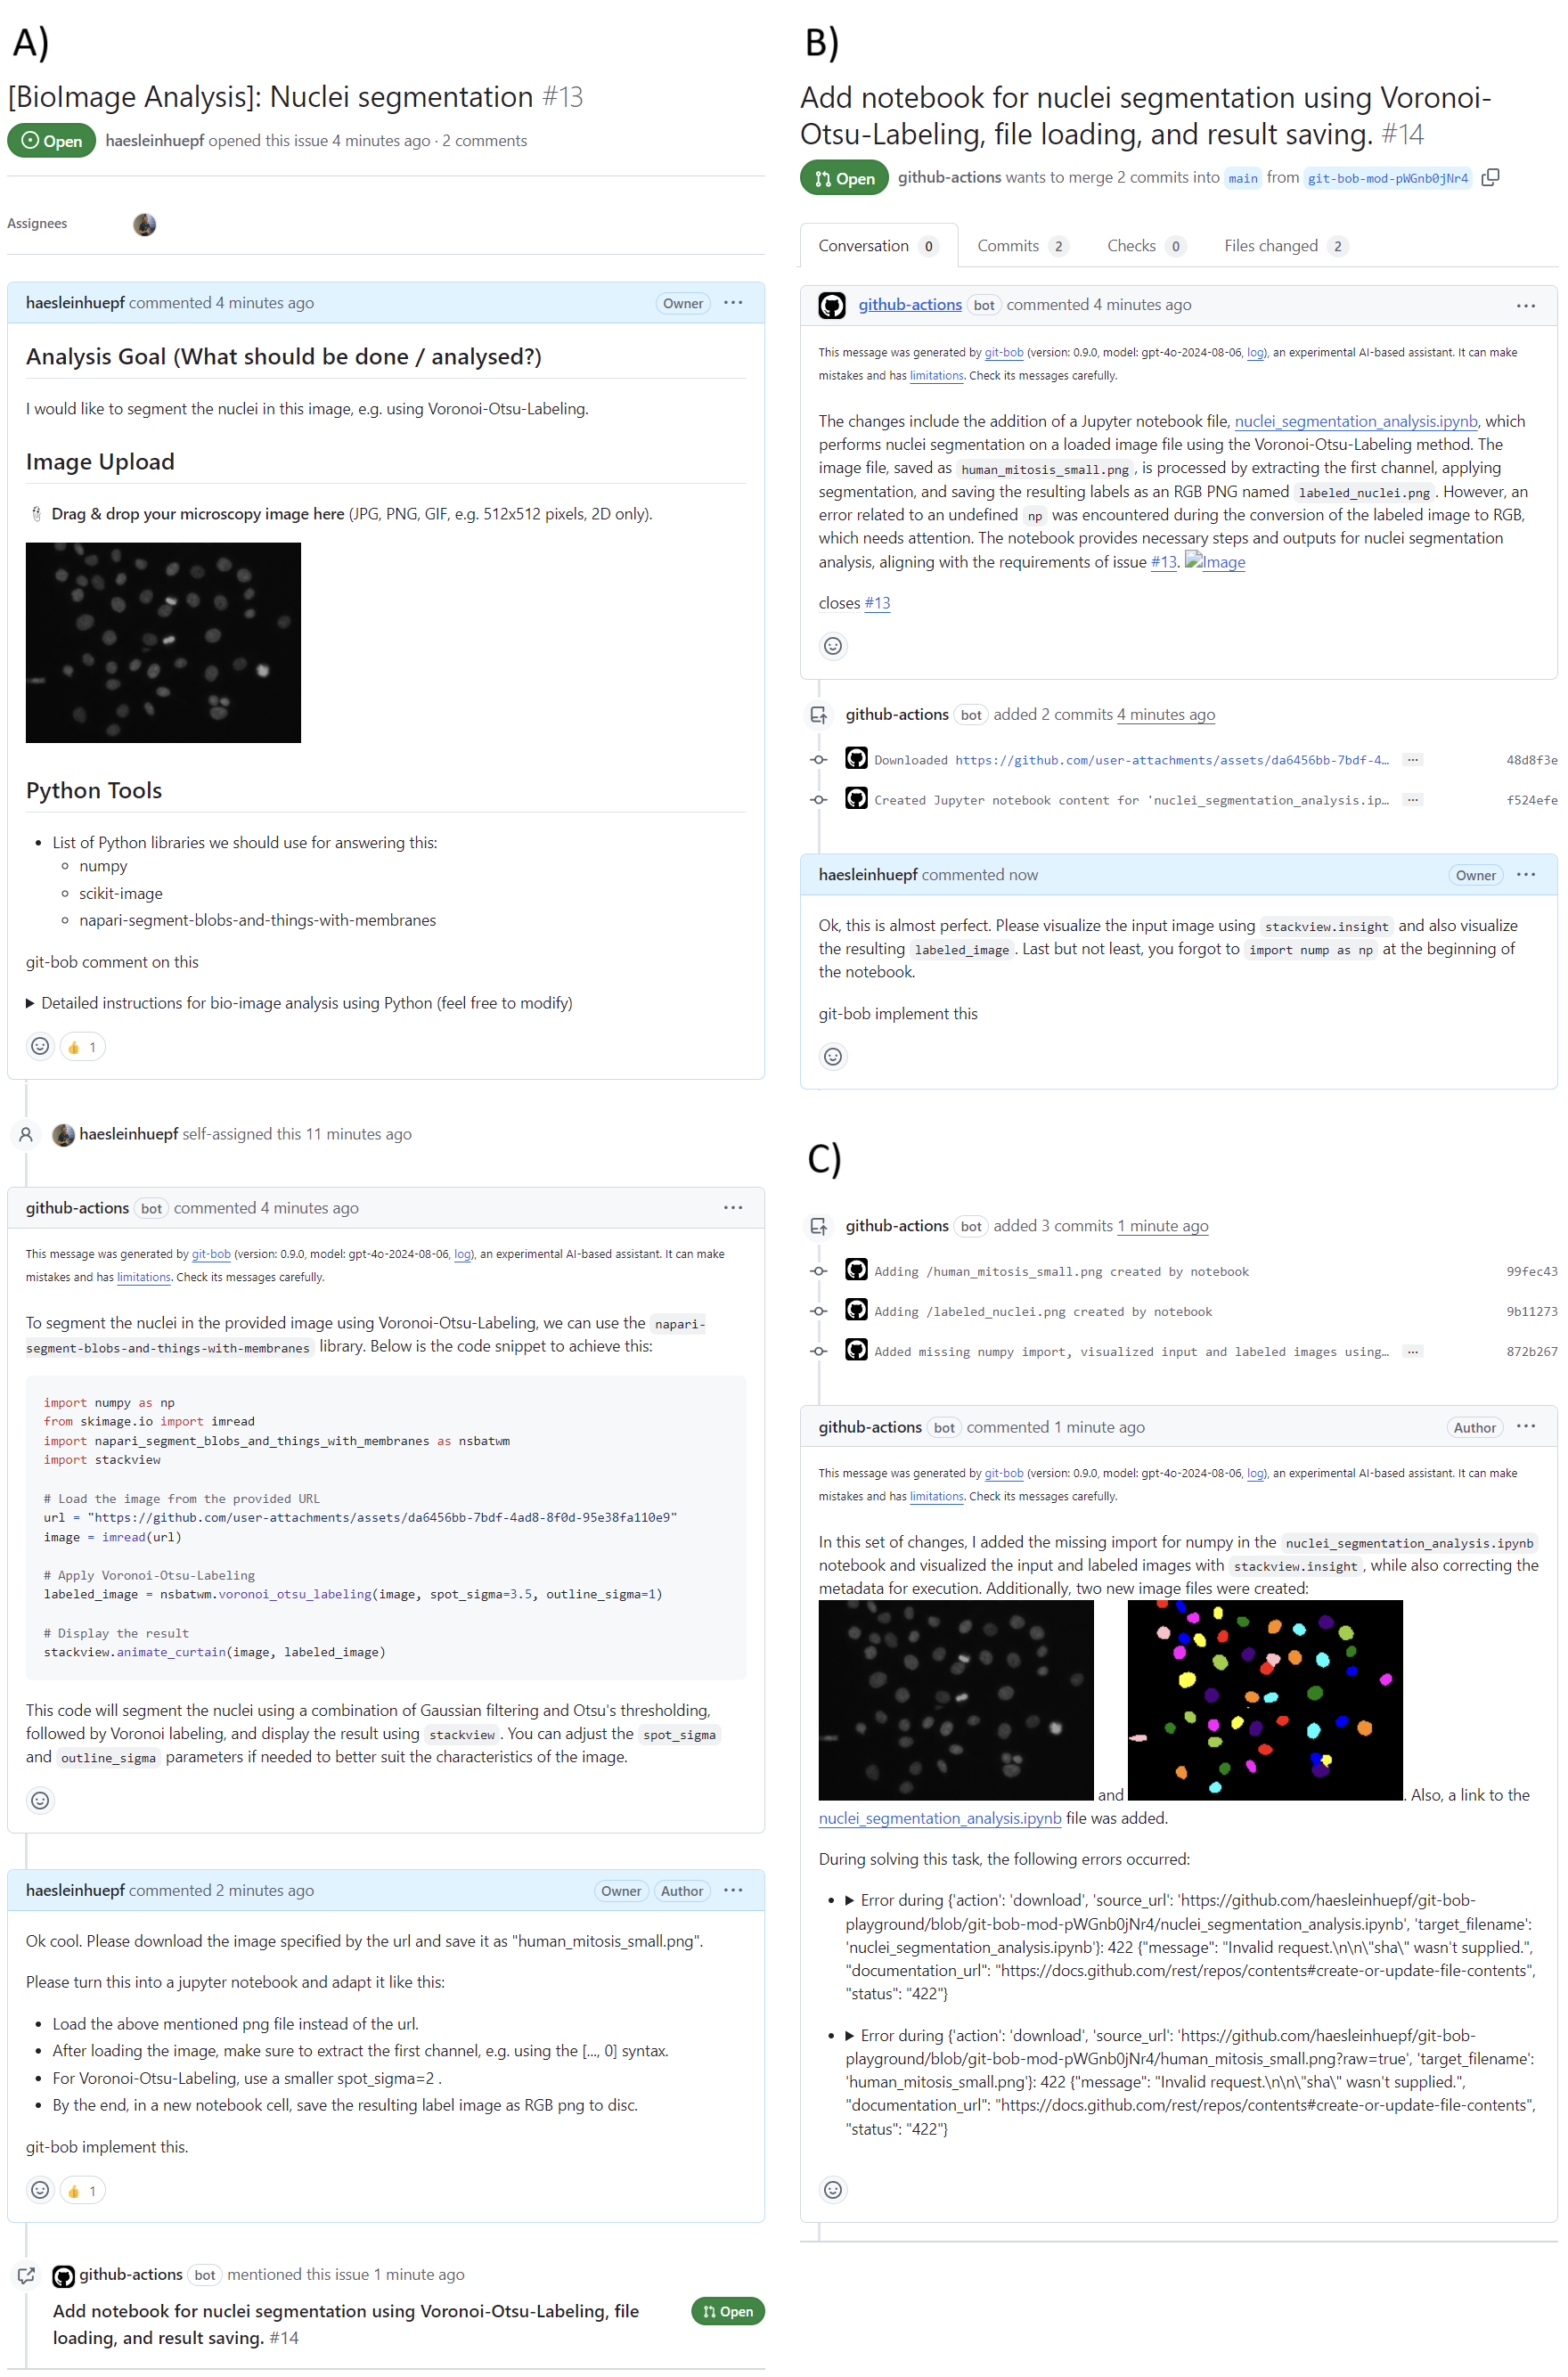
\includegraphics[width=0.82\textwidth]{example_interaction.png}
\caption{Use-case example for the interaction with git-bob: After creating a GitHub issue, optionally including upload of an example image, the AI-assistant and the human exchange about how to process the data (A). Once they concluded to implement the solution, a GitHub pull-request is sent (B) containing the programmed solution as files in the repository. Also here, human and AI-assistant can continue discussing and modify the solution until the example is satisfactory.  The entire discussion and corresponding code can be read online: \url{https://github.com/haesleinhuepf/git-bob-playground/issues/13} and \url{https://github.com/haesleinhuepf/git-bob-playground/pull/14}
\newline
\newline
}
\label{fig:example_interaction}
\end{figure*}

\section{Supplementary material}
\setcounter{figure}{0} 
\renewcommand{\thefigure}{S\arabic{figure}}




\begin{figure*}[h]
\centering
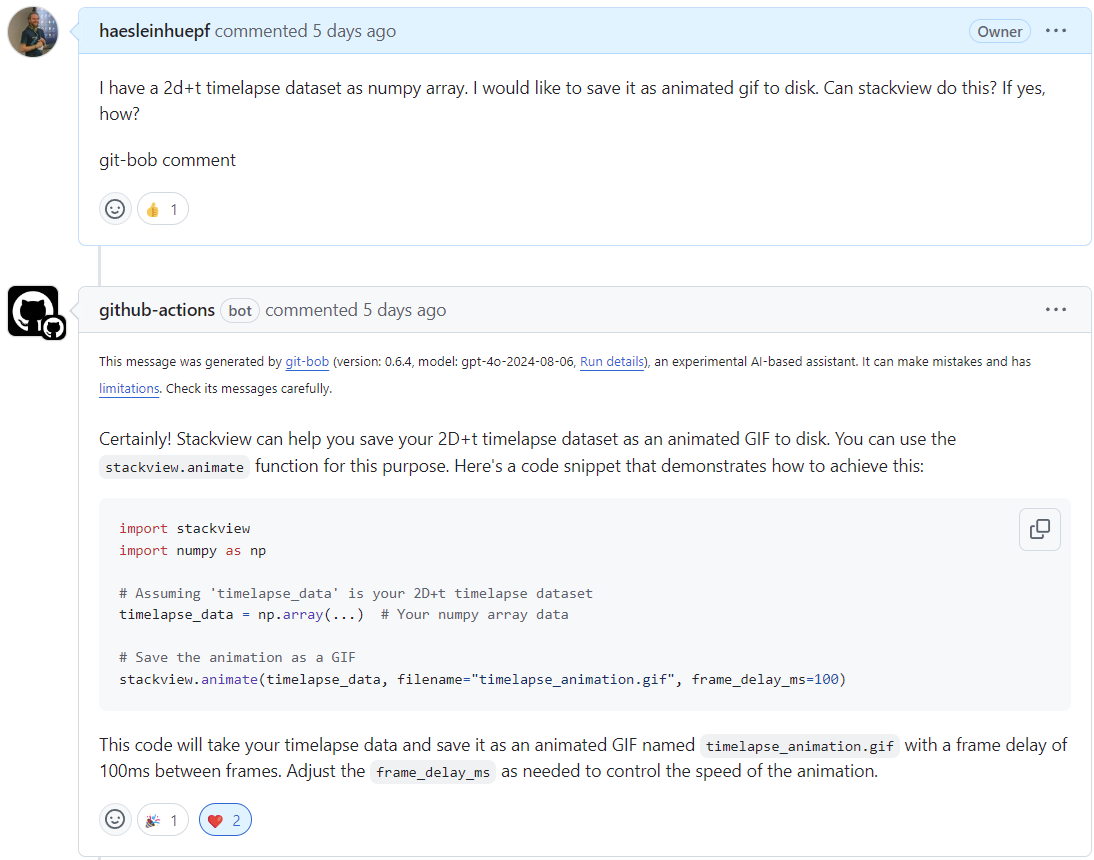
\includegraphics[width=0.82\textwidth]{example_supporting_users.png}
\caption{Use-case example for supporting users: The assistant can be configured to act as expert on a specific Python library and answer user questions. The entire discussion and corresponding code can be read online: \url{https://github.com/haesleinhuepf/stackview/issues/79}
\newline
\newline
}
\label{fig:examplesupportingusers}
\end{figure*}


\begin{figure*}[h]
\centering
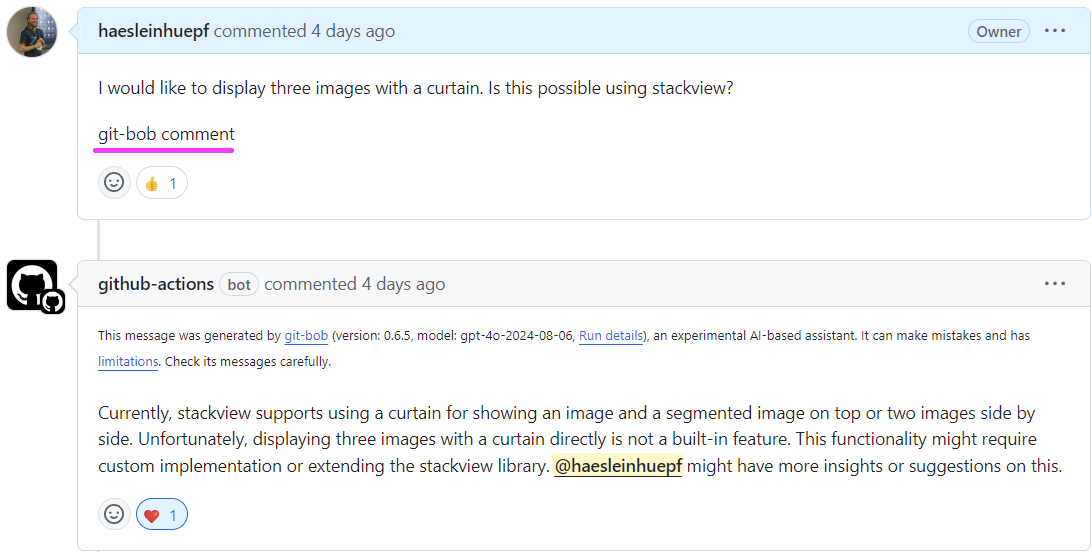
\includegraphics[width=0.82\textwidth]{example_supporting_users2.png}
\caption{Use-case example for asking an expert: The answer to the question shown here is "No", but this is nowhere written in the documentation or the configuration of the assistant. In this case the assistant is not sure, and it can be configured to forward a question to a maintainer of the library where the question arrived. The entire discussion and corresponding code can be read online: \url{https://github.com/haesleinhuepf/stackview/issues/80}
\newline
\newline
}
\label{fig:examplesupportingusers2}
\end{figure*}


\begin{figure*}[h]
\centering
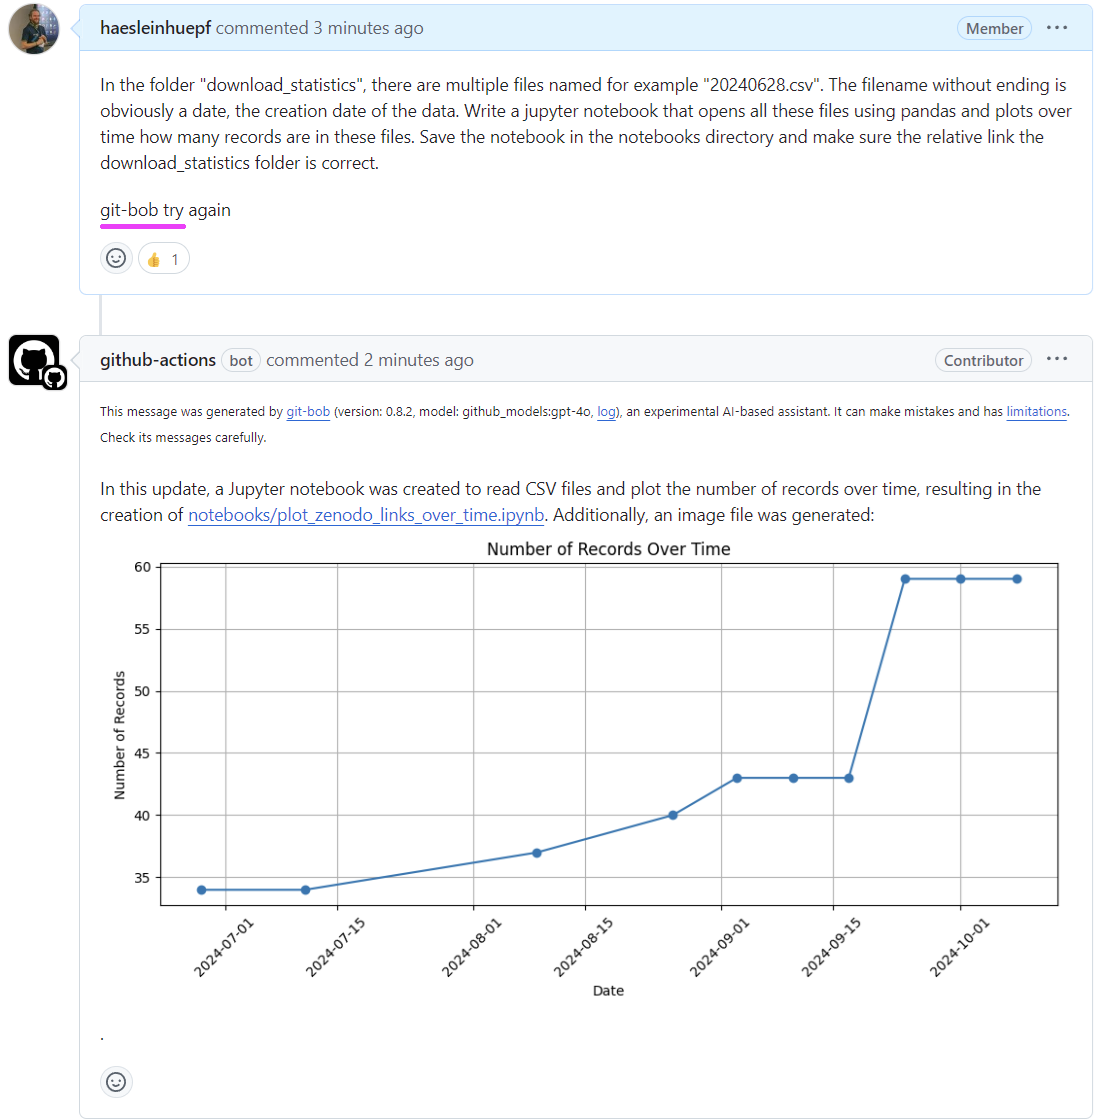
\includegraphics[width=0.82\textwidth]{example_plotting.png}
\caption{Use-case example for plotting data: After explaining the assistant the folder structure of the project, it generates code for parsing a folder of CSV files and plotting results. The entire discussion and corresponding code can be read online: \url{https://github.com/NFDI4BIOIMAGE/training/issues/250}
\newline
\newline
}
\label{fig:exampleplotting}
\end{figure*}


\begin{figure*}[h]
\centering
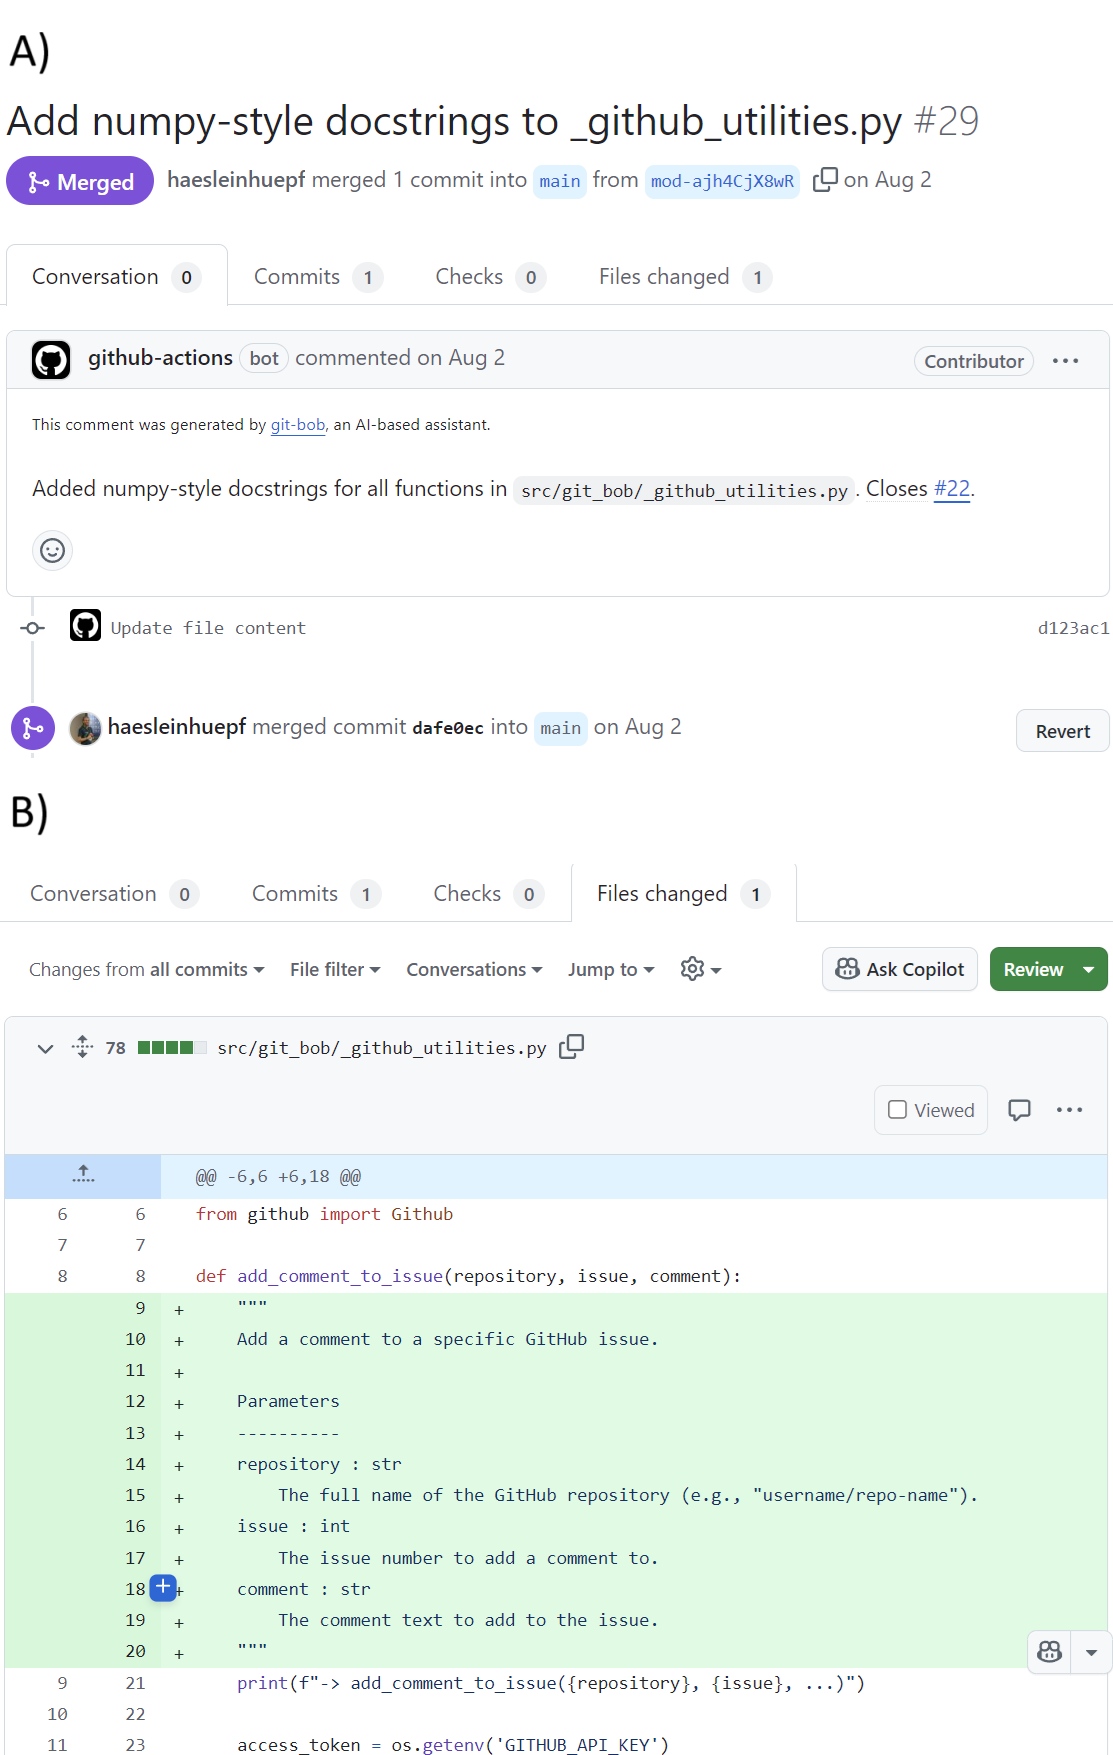
\includegraphics[width=0.82\textwidth]{example_add_documentation.png}
\caption{Use-case example for adding and revising documentation in code: git-bob was used to partially write the code documentation of its own code. When asked to add documentation in a specific format, it sent a pull-request (A) and the human could inspect the code modifications (B, excerpt) before mergin the code into the project's code base. The entire discussion and corresponding code can be read online: \url{https://github.com/haesleinhuepf/git-bob/pull/29}
\newline
\newline
}
\label{fig:example_add_documentation}
\end{figure*}




\begin{figure*}[h]
\centering
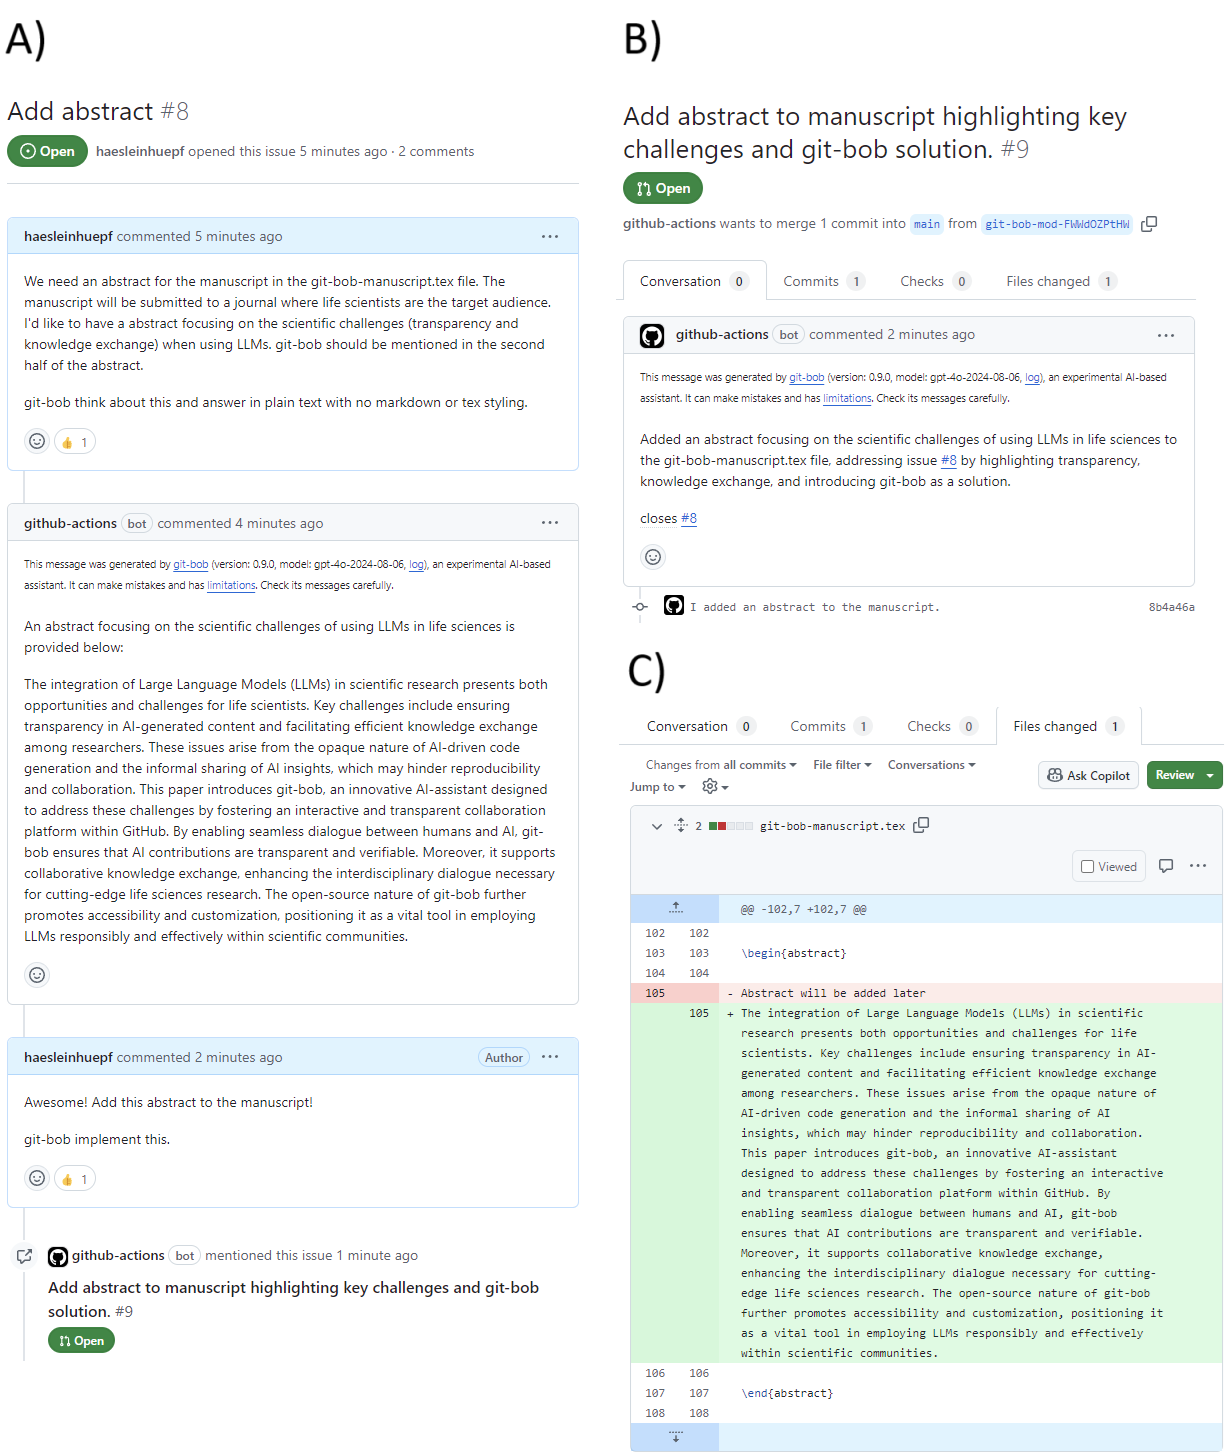
\includegraphics[width=0.82\textwidth]{example_abstract_generation.png}
\caption{Use-case example for working on scientific manuscripts: After a first draft of the manuscript was written, git-bob was asked to formulate an abstract (A). The abstract was then submitted as pull-request with a short description (B). The human can also review and potentially modify the proposed text in this online interface (C). The entire discussion can be read online: \url{https://github.com/haesleinhuepf/git-bob-manuscript/issues/8} and \url{https://github.com/haesleinhuepf/git-bob-manuscript/pull/9}.
\newline
\newline
}
\label{fig:xample_abstract_generation}
\end{figure*}

\end{document}
%%%%%%%%%%%%%%%%%%%%%%%%%%%%%%%%%%%%%%%%%%%%%%%%%%%%%%%%%%%%%%%%%%%%%%
